\textbf{Uso del diagrama de dispersión en el análisis de grupos}

El diagrama de dispersión (\textit{scatter plot}) es una de las herramientas visuales más fundamentales y poderosas en las fases exploratorias y evaluativas del análisis de grupos (\textit{clustering}). Su propósito es proyectar un conjunto de datos en un espacio bidimensional (o tridimensional) basado en dos o tres características continuas. 

En el contexto del \textit{clustering}, el diagrama de dispersión ayuda de las siguientes maneras:
\begin{itemize}
    \item \textbf{Identificación de la estructura natural:} Permite a simple vista determinar si los datos tienen agrupaciones inherentes, cuántos grupos posibles hay (estimación de $k$), y qué forma geométrica tienen dichos grupos (ej. esféricos, alargados, anillos concéntricos).
    \item \textbf{Selección del algoritmo adecuado:} Si el diagrama muestra grupos esféricos y densos, algoritmos basados en centroides como \textit{K-means} serán adecuados. Si muestra formas irregulares o no lineales, se requerirán métodos basados en densidad como \textit{DBSCAN} o agrupación espectral.
    \item \textbf{Evaluación de resultados:} Después de aplicar un algoritmo de clustering, se puede colorear el diagrama de dispersión según las etiquetas de grupo asignadas por el modelo, permitiendo verificar visualmente la calidad de la separación y la cohesión de los grupos.
\end{itemize}

\textbf{Ejemplo Ilustrativo}

Supongamos que una empresa de comercio electrónico desea segmentar a sus clientes para campañas de marketing. Se extraen dos variables principales: \textbf{Ingreso Anual (en miles de \$)} y un \textbf{Índice de Gasto} (puntuación del 1 al 100 basada en el comportamiento de compra).

\begin{figure}[H]
    \centering
    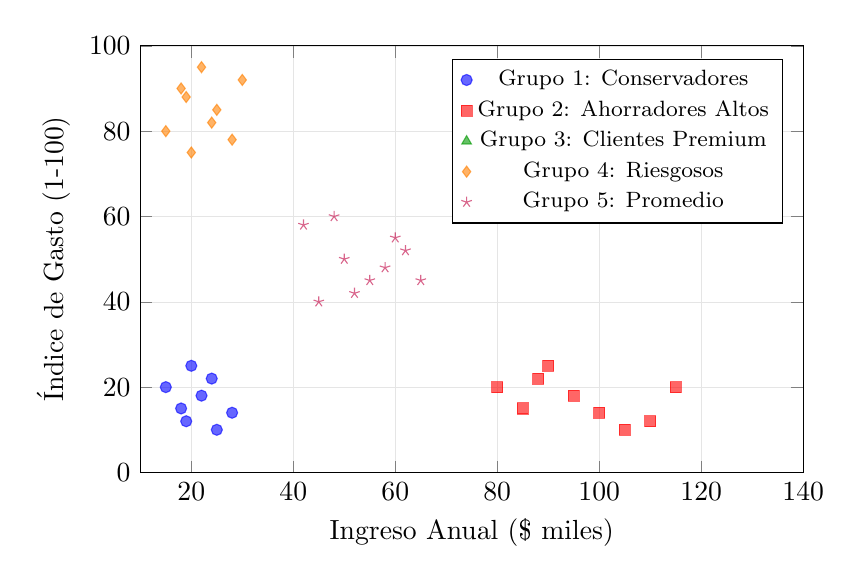
\begin{tikzpicture}
        \begin{axis}[
            width=10cm,
            height=7cm,
            xlabel={Ingreso Anual (\$ miles)},
            ylabel={Índice de Gasto (1-100)},
            xmin=10, xmax=140,
            ymin=0, ymax=100,
            grid=both,
            grid style={line width=.1pt, draw=gray!20},
            legend pos=north east,
            legend style={font=\footnotesize}
        ]
        
        % Cluster 1: Ingresos bajos, gastos bajos (Ahorradores)
        \addplot[only marks, mark=*, color=blue, opacity=0.6] coordinates {
            (15, 20) (18, 15) (20, 25) (25, 10) (22, 18) (19, 12) (24, 22) (28, 14)
        };
        \addlegendentry{Grupo 1: Conservadores}
        
        % Cluster 2: Ingresos altos, gastos bajos (Cuidadosos)
        \addplot[only marks, mark=square*, color=red, opacity=0.6] coordinates {
            (80, 20) (85, 15) (90, 25) (105, 10) (95, 18) (110, 12) (88, 22) (100, 14) (115, 20)
        };
        \addlegendentry{Grupo 2: Ahorradores Altos}
        
        % Cluster 3: Ingresos altos, gastos altos (Objetivo ideal)
        \addplot[only marks, mark=triangle*, color=green!60!black, opacity=0.6] coordinates {
            (75, 80) (85, 90) (90, 75) (105, 85) (95, 95) (110, 88) (88, 82) (100, 78) (120, 92) (80, 85)
        };
        \addlegendentry{Grupo 3: Clientes Premium}
        
        % Cluster 4: Ingresos bajos, gastos altos (Derrochadores)
        \addplot[only marks, mark=diamond*, color=orange, opacity=0.6] coordinates {
            (15, 80) (18, 90) (20, 75) (25, 85) (22, 95) (19, 88) (24, 82) (28, 78) (30, 92)
        };
        \addlegendentry{Grupo 4: Riesgosos}
        
        % Cluster 5: Promedio
        \addplot[only marks, mark=star, color=purple, opacity=0.6] coordinates {
            (45, 40) (50, 50) (55, 45) (60, 55) (48, 60) (52, 42) (58, 48) (62, 52) (42, 58) (65, 45)
        };
        \addlegendentry{Grupo 5: Promedio}

        \end{axis}
    \end{tikzpicture}
    \caption{Diagrama de dispersión de clientes: Ingreso Anual vs. Índice de Gasto. Se evidencian visualmente 5 grupos distintos.}
    \label{fig:scatter_clustering}
\end{figure}

Al graficar estos datos en un diagrama de dispersión (Figura \ref{fig:scatter_clustering}), el analista puede observar de inmediato que los datos tienden a formar cinco agrupaciones bien diferenciadas. Sin el diagrama, observar únicamente una tabla con cientos de filas de ingresos e índices de gasto haría casi imposible notar esta estructura pentagonal subyacente. Esta visualización previa justifica la elección de usar, por ejemplo, el algoritmo K-means con $K=5$ para etiquetar formalmente a los clientes y luego diseñar estrategias de marketing específicas para cada grupo (ej. promociones de lujo para el "Grupo 3").
